\documentclass[11pt,a4paper]{article}

\usepackage[margin=1in]{geometry}
\usepackage{amsmath,amssymb,amsthm}
\usepackage{graphicx}
\usepackage[hidelinks]{hyperref}
\usepackage{booktabs}
\usepackage{enumitem}
\usepackage{tikz}
\usepackage{xcolor}
\usepackage{titlesec}
\usepackage[expansion=false]{microtype}
\usepackage{caption}
\usetikzlibrary{arrows.meta,positioning,fit,backgrounds,shapes.geometric,shadows}

\definecolor{abstrcol}{HTML}{2C5F8A}
\definecolor{numcol}{HTML}{D4850A}
\definecolor{boxbg}{HTML}{F5F5F5}

\titleformat{\section}{\Large\bfseries\color{abstrcol}}{\thesection}{1em}{}
\titleformat{\subsection}{\large\bfseries}{\thesubsection}{1em}{}

\newcommand{\abstr}[1]{\textcolor{abstrcol}{#1}}
\newcommand{\numr}[1]{\textcolor{numcol}{#1}}

\title{Operator and Representation Layers for Computational Materials Science:\\
       Principles and First-Demonstration Plan}
\author{G. Barbalinardo \\
        \small University of California, Davis}
\date{\today}

\begin{document}

\maketitle

\begin{abstract}
This document records the design of a typed operator/representation framework for computational materials science
workflows, organized around a small set of principles. Workflows are directed
acyclic graphs of \emph{operator physics states} connected by \emph{operator operations}, and
concrete numerical results are \emph{representations}---typed projections of operator states
into a discretization scheme. The operator root is the \emph{Born--Oppenheimer
potential} of a material, expanded as a Taylor series in atomic displacements; force constants
of every order are derived states obtained by extracting derivatives of this root and truncating
the expansion at a chosen order. Every state carries a provenance chain that records the
operations along its path; every representation carries a discretization scheme. Approximation
and discretization errors live in disjoint type universes and compose along graph edges; the
machinery for tracking error formulas symbolically and composing them across the graph is
designed but its full implementation is deferred to Phase 2. As a first demonstration, three
established lattice thermal-transport codes (kaldo, phono3py, ShengBTE) are reframed as distinct
representations of a single operator DAG, with cross-code reconciliation at canonical
intermediate states as the Phase 1 deliverable. Phase 1 stubs the upstream operations that
produce force constants from the potential---declaring the relevant operator types and provenance
labels but not modeling them in detail---so that Phase 2 can elaborate the upstream without
restructuring the framework. The document is intended as the working architectural reference for
the \texttt{openmaterials-ai} project; it covers each architectural decision, the alternatives
considered, and what we deferred.
\end{abstract}

\tableofcontents

\bigskip

\section{Principles}
\label{sec:principles}

The operator layer is built on a small set of commitments. They are stated here without
their alternatives or justifications; supporting definitions follow in later sections.

\begin{enumerate}[leftmargin=2.5em, itemsep=0.4em]
  \item \textbf{Two worlds, one bridge.} The operator layer keeps the operator physics world
        (typed states, operator operations, approximation errors) strictly separate from
        the numeric world (discretized arrays, computed values, discretization errors).
        They are connected by exactly one bridge: the representation functor.

  \item \textbf{Operator states are unit-free.} Dimensionful quantities (frequency,
        energy, length, time) exist at the operator layer, but specific unit choices
        (THz vs eV vs rad/s, \AA{} vs Bohr) do not. Unit choice belongs to the
        representation and is declared by the adapter that produced it; the framework
        normalizes to a canonical unit before any cross-representation comparison.

  \item \textbf{The atom is a operator operation.} The atomic unit of meaning is a typed
        transformation between operator states, not an instruction in an input file or an
        algorithm. Every operation carries a \emph{operator formula}---a sympy expression
        (closed-form output) or sympy.Eq (implicit equation defining the output)---stating
        what it computes. The formula is the operator claim, machine-readable and
        Lean-projectable, against which adapter conformance can be checked.

  \item \textbf{States are typed witnesses; nodes are Observables or HiddenStates.}
        A state is the typed claim that a operator physics object exists with a
        particular history. The operator layer splits states into two structural kinds:
        \emph{Observables} (gauge-invariant, first-class, required to agree across
        adapters) and \emph{HiddenStates} (gauge-dependent intermediate scaffolding
        whose per-element values reflect basis / phase / BZ-summation choices the
        framework does not pin down). Each state declares fields, and each field has an
        index signature (e.g.\ $\omega(\mathbf{q},\nu)$ has indices $(\mathbf{q}, \nu)$;
        $\kappa^{\alpha\beta}$ has $(\alpha, \beta)$). Numerical content lives in the
        representation, separate from the witness.

  \item \textbf{Workflows are directed acyclic graphs.} A workflow is a graph of states
        connected by operations, not a linear sequence. Cross-code comparison reduces
        to graph alignment over the same operator template.

  \item \textbf{Identity is type plus provenance.} A operator state is identified by its
        physics type and the ordered chain of operations that produced it. Two states
        with the same type but different histories are different states.

  \item \textbf{Operation identity is parameterized.} An operation is identified by its
        name together with the parameters that affect physics. Different physics-affecting
        parameter values produce different operations and therefore different output
        states. Function-family parameterizations (e.g., Gaussian broadening by standard
        deviation vs.\ by half-width) are canonicalized at the operator layer to a single
        choice; adapters translate to their internal convention.

  \item \textbf{Discretization belongs to representation.} Mesh densities, supercell
        sizes, displacement steps, and broadenings live on the representation, not on
        the operator state. Convergence is a relationship between a operator state and
        a family of its representations.

  \item \textbf{Cross-code agreement is required at Observable nodes only.} Two
        adapters' representations of an Observable must agree (after unit and
        convention conversion) to within the observable's declared tolerance.
        Representations of a HiddenState are not cross-code comparable per-element;
        the operator layer's \texttt{compare} returns the status \texttt{NOT\_COMPARABLE}
        and reports residuals as diagnostic information only. To make a HiddenState
        cross-code comparable, contract it into an Observable (e.g., per-mode
        $\Gamma_{q\nu}$ is a HiddenState; $\sum_{q\nu}\Gamma$ contracted via the
        BZ sum is an Observable that does agree).

  \item \textbf{Errors are designed-for.} Approximation errors live on operations;
        discretization errors live on representations. The type system reserves slots
        for both; operator composition of error formulas is a Phase~2 capability.

  \item \textbf{The operator root is the potential.} Every representation in the framework
        ultimately traces back to the Born--Oppenheimer potential of the material. Force
        constants of every order are derived states obtained by extracting derivatives of
        the potential and truncating the Taylor expansion. The upstream is stubbed in
        Phase~1.

  \item \textbf{Sources are produced by nullary operations.} Source states (the
        potential, but also temperature, lattice constant, etc.)\ are the outputs of
        nullary \texttt{provide\_*} operations rather than nodes with empty provenance.
        This unifies the DAG: every node is the output of some operation, and the
        operator layer has no special ``input'' category. The representation of a source
        state carries the externally supplied value (e.g., $T = 300\,\mathrm{K}$); the
        operation is just a structural tag.

  \item \textbf{Lean-compatible by structure.} The operator layer is implemented in Python
        but designed so that its types transliterate cleanly into Lean. Three disciplines
        protect this option: closed unions for physics types, no Python-encoded physics
        invariants, operation parameters always recorded in output state metadata.
       
\end{enumerate}

\bigskip


\section{Background and Motivation}
\label{sec:motivation}

Modern computational materials science has many codes, many workflows, and many opinions about how
to compose them. Despite a generation of effort on workflow managers (\textsc{AiiDA}, \textsc{Atomate},
\textsc{FireWorks}, \textsc{Atomate2}, \textsc{Aflow}), one quality is still missing: a workflow
should expose, as typed and composable data, \emph{the physics it computes}.

Today the standard unit of shared meaning between codes is the \emph{input file}: an ordered
sequence of instructions that, together with a particular code's internal logic, produces an
output. This unit is opaque to two questions:

\begin{itemize}[leftmargin=2em]
  \item \textbf{Given a result, what physical assumptions and approximations does it embed?}
        An input file declares parameters but not their meaning. A k-mesh is just a triple of
        integers; the relationship between that mesh and the convergence of the integrated
        observable is not part of the file.
  \item \textbf{Given two results from two codes, where exactly do they diverge?} Identical force
        constants run through kaldo and through ShengBTE typically yield slightly different
        thermal conductivities. The difference is not localized to a particular operation, even
        though---in principle---it is the result of distinct computational choices at specific
        steps.
\end{itemize}

A previous attempt of ours, \texttt{MaterialsCodeGraph} (MCG), addressed parts of this gap by
treating each instruction in an input file as the atomic unit of a knowledge graph and tracking
inputs, parameters, and outputs at that level. MCG's tool-encapsulation principle (all tool
knowledge in YAML/Markdown configs, all code generic over tool) was the right design at that
level of abstraction. But the level of abstraction itself is too low: an instruction in an input
file is a syntactic unit, not a semantic one. It tells you what a code is told to do, not what
\emph{physics} the code thereby computes. Two codes that compute the phonon dispersion via
diagonalization of the dynamical matrix express that operation as different instructions; yet
they perform the same physics. A graph indexed by instructions sees them as two unrelated tasks.

\medskip

The operator layer proposed here \emph{starts from the physics} and treats input files as derived
artifacts. The atomic unit is no longer an instruction; it is a \emph{operator operation} between
typed physics states. The states are the load-bearing entities: a state is what changes when an
operation is applied, and a workflow is the graph that records those state transitions. Concrete
numerical computation is then a separate, typed projection of the operator workflow into a
discretization scheme.

This is a deliberate departure from the input-file paradigm. We argue below that it pays for the
extra abstraction with three concrete returns: cross-code reconciliation at canonical intermediate
states, derived (rather than empirical) error bounds on computed observables, and a clean
foundation for future formal verification.

\section{Architectural Principle: Two Worlds, One Bridge}
\label{sec:principle}

The single most important design decision is a strict separation between two type universes:

\begin{itemize}[leftmargin=2em]
  \item \abstr{\textbf{The operator world}} holds typed physics states (Hamiltonians, dispersion
        relations, scattering rates, distribution functions, partition functions) and operator
        operations between them. Errors here are \emph{approximation errors}---the $O(\cdot)$
        terms introduced by truncating perturbation series, linearizing equations, or imposing
        physical assumptions such as the Born--Oppenheimer or harmonic approximation. The
        operator world contains no numerical content. Two operator states that differ only in
        their numerical estimates are the same operator state; two operator states that differ
        in the chain of approximations leading to them are different operator states.
  \item \numr{\textbf{The numeric world}} holds discretized realizations of operator states:
        arrays sampled on finite grids, mode-resolved quantities at finite k-meshes,
        distributions evaluated at finite temperature. Errors here are \emph{discretization
        errors}---the $O((1/N)^k)$ or $O(h^k)$ terms introduced by sampling a continuum quantity
        on a finite scheme. The numeric world contains no operator content; it does not know
        what theory the numbers are estimates of.
\end{itemize}

The two worlds are connected by exactly one bridge, the \emph{representation functor}, which
takes (i) a operator state and (ii) a discretization scheme and produces a numeric
representation. Approximation errors compose in the operator world along provenance chains;
discretization errors compose in the numeric world along execution graphs; the two combine only
at representation time, where the total error of a numerical result decomposes into its operator
and numeric contributions.

This separation is load-bearing. It is also somewhat unusual. Most computational physics codes
mix the two worlds: a ``Hamiltonian'' object in such a code is sometimes a typed mathematical
operator and sometimes a 4-D \texttt{numpy} array. The operator layer refuses to do this. If you are
holding a Hamiltonian, you know which world you are in and you cannot
accidentally mix the two. This refusal is what makes errors composable, theorems statable, and
cross-code comparisons well-defined.

\subsection{The full chain: two layers plus the external codes}
\label{ssec:two-layer-chain}

In implementation terms, the project has \emph{exactly two layers} under its
own control plus the external physics codes that produce numerical data.
Nothing else is a layer: tests, visualization, and experiment scripts are
supporting infrastructure.

\paragraph{Layer 1 --- operator.} Types, declarations, formulas, gauges.
Machinery in \texttt{omai.operator} (the \texttt{State} and
\texttt{Operation} types, \texttt{Field}, \texttt{Dimension},
\texttt{GaugeAction}, \texttt{SymmetryGroup}, \texttt{validate\_dag});
domain instances in \texttt{omai.thermal\_transport.operator} (the
46-node, 47-edge DAG with sympy formulas on each edge, gauge actions).
No values, no units, no per-code knowledge.

\paragraph{Layer 2 --- representation.} Per-code declarations plus the
runtime that operates on actual code outputs. Machinery in
\texttt{omai.representation} (the \texttt{StateAdapterSpec} and
\texttt{OperationAdapterSpec} types, \texttt{Unit} and unit conversions,
the \texttt{Representation} runtime data class, \texttt{compare()} with
its five-status verdicts); domain instances in
\texttt{omai.thermal\_transport.represented} (one file per code:
\texttt{kaldo.py}, \texttt{phono3py.py}).

\paragraph{External codes.} kaldo, phono3py, ShengBTE: do the actual
physics computation in their own native code, output arrays in their
native units and conventions.

\paragraph{The chain in motion.} A typical cross-code verification flows
through these layers like this:

\begin{enumerate}[leftmargin=2em, itemsep=0.2em]
  \item User invokes the codes externally (e.g.\ kaldo and phono3py),
        which produce raw output arrays in their own formats.
  \item User wraps each array via \texttt{represent(spec, field\_name,
        array)}: this validates the field exists on the operator state
        and produces a \texttt{Representation} object tagged with the
        right adapter spec.
  \item User calls \texttt{compare(m\_a, m\_b)}. \texttt{compare} consults
        the operator layer for the cross-code factor (units +
        conventions), applies it, optionally contracts, and consults the
        operator layer again for the state's gauge kind to decide whether
        an \textsc{Agree}/\textsc{Disagree} verdict is even meaningful or
        the comparison is \textsc{Not\_Comparable}.
  \item User gets a \texttt{RepresentationComparisonResult} with status, residuals,
        and the applied factor.
\end{enumerate}

\noindent No additional layers, no other indirection. The two
two layers expose their content in matched pairs (machinery
in \texttt{omai/<layer>/}, domain instances in
\texttt{omai/<domain>/<layer>/}), and the codes attach at the edge.

\medskip

\section{Formal Definitions}
\label{sec:defs}

We collect the formal definitions implied by the decisions above.

\subsection{Operator state}

A operator state $s$ is unit-free: its physics type carries the dimension of any
quantity it represents (a frequency, an energy density, a tensor of given rank), but no
unit choice. Numerical content and units appear only at representation time.

\medskip

A operator state $s$ is a tuple $(\kappa, \tau, \pi, F)$ where:
\begin{itemize}[leftmargin=2em]
  \item $\kappa \in \{\textsc{Observable}, \textsc{HiddenState}\}$ is the
        \emph{gauge-invariance kind}: Observables are gauge-invariant and cross-code
        comparable; HiddenStates carry gauge freedom (eigenvector phase, BZ-summation
        choice, degenerate-subspace rotation, …) that the operator layer doesn't pin down,
        so their per-element values differ across adapters by design;
  \item $\tau$ is a \emph{physics type} drawn from a finite registry. Derived types in
        the thermal-transport scope include \texttt{ForceConstants[order=$n$]},
        \texttt{DynamicalMatrix}, \texttt{Frequency}, \texttt{Eigenvectors},
        \texttt{GroupVelocity}, \texttt{HeatCapacity}, \texttt{Linewidth},
        \texttt{MeanFreeDisplacement}, \texttt{ThermalConductivity}; sources include
        \texttt{Potential}, \texttt{Temperature}. Some types are further parameterized
        by upstream operation choices (e.g., \texttt{ThermalConductivity[bte\_solver=
        rta]} is a HiddenState since RTA's $1/\Gamma$ non-linearity breaks gauge
        invariance, whereas \texttt{ThermalConductivity[bte\_solver=direct\_inverse]}
        is an Observable because the full LBTE preserves it);
  \item $\pi$ is the \emph{provenance}: an ordered list $[\mathcal{O}_1, \mathcal{O}_2,
        \ldots, \mathcal{O}_n]$ of operator operations whose composition produced $s$.
        Provenance is never empty---source states have a single nullary operation
        (\texttt{provide\_potential}, \texttt{provide\_temperature}, \ldots);
  \item $F = (f_1, f_2, \ldots)$ is the state's tuple of \emph{fields}. Each field has
        a name, a dimension (frequency, energy, length, …), and an index signature
        (e.g., $\omega$ has indices $(\mathbf{q}, \nu)$; $v$ has $(\alpha, \mathbf{q},
        \nu)$; $\kappa$ has $(\alpha, \beta)$).
\end{itemize}
Two operator states are equal iff their names match. The composed approximation error
on $s$ (a Phase 2 capability) would be
\begin{equation}
  \epsilon_{\text{approx}}(s) = \mathrm{compose}\bigl(\epsilon_{\mathcal{O}_1},\, \epsilon_{\mathcal{O}_2},\, \ldots,\, \epsilon_{\mathcal{O}_n}\bigr).
\end{equation}

\paragraph{Source versus derived states.} Operator states fall into two kinds, both
produced by some operation:
\begin{itemize}[leftmargin=2em]
  \item \emph{Source states} are the outputs of \emph{nullary} operations
        (\texttt{provide\_potential}, \texttt{provide\_temperature}, \ldots): operations
        with no operator-state inputs. They are empirical inputs (lattice constant,
        temperature, pressure, applied field), the operator \texttt{Potential} itself
        (Phase 1 stubs the upstream of the potential), or measured observables (a
        thermal conductivity reported from a TDTR experiment, a Raman peak). The
        representation of a source state carries the externally supplied value (e.g.,
        $5.43\,\textup{\AA}$ for the lattice constant of silicon, or $T = 300\,\text{K}$);
        its discretization scheme is trivial (a singleton choice rather than a refinable
        mesh) but its error is still meaningful (experimental uncertainty, or
        definitional precision).
  \item \emph{Derived states} are the outputs of operations that consume one or more
        upstream states. Examples: \texttt{ForceConstants[order=$n$]} (derived from
        \texttt{Potential} via \texttt{compute\_force\_constants[order=$n$]}, currently
        stubbed), \texttt{Frequency} and \texttt{Eigenvectors} (multi-output of
        \texttt{compute\_dispersion}), \texttt{Linewidth},
        \texttt{MeanFreeDisplacement}, the computed $\kappa$.
\end{itemize}
Both kinds follow the same machinery for representation. The unification of source and
derived states under the same ``output of an operation'' rule answers several otherwise
awkward cases: empirical inputs (``where does the lattice constant live?''), experimental
observables (``how does a measured $\kappa(T)$ enter the framework?''), and the unmodeled
operator root in Phase 1 (``what is the silicon potential, before we differentiate
it?''). All three are representations of source states whose provenance is a single
nullary operation; the second is what makes the unified theory--experiment comparison
framework native rather than bolted on; the third is how Phase 1 stubs the upstream of
\texttt{Potential} without yet modeling it in detail.


\paragraph{What ``witness-as-state'' means, concretely.}

The phrase \emph{witness-as-state} comes from the Curry--Howard correspondence in type theory:
a typed value is read as evidence (a ``witness'') for a proposition. We borrow the intuition
without borrowing the formal proof obligations. In this framework a state is not the data it
contains; it is the \emph{claim} that something exists, expressed in a typed form rich enough
to carry meaning.

Concretely, three layers are conflated in most computational physics codes; the operator layer keeps
them apart:

\begin{enumerate}[leftmargin=2em]
  \item \textbf{The proposition} -- ``the phonon dispersion of crystalline silicon under the
        harmonic approximation, derived by truncating the Born--Oppenheimer Taylor expansion at
        second order, exists as a function $\omega(\mathbf{q}, \nu)$ from the Brillouin zone to
        positive reals.''
  \item \textbf{The witness} -- a typed object \texttt{s = (Dispersion, $\pi$)} that records
        precisely this claim. The physics type \texttt{Dispersion} encodes the kind of object
        being asserted to exist; the provenance $\pi$ records the chain of operations
        (extraction, truncation, Fourier transform, eigendecomposition) that produced it. The
        witness carries no numerical content; it is the assertion that such an object exists
        with this history.
  \item \textbf{The representation} -- a tuple $(s, \Sigma, x, \epsilon_{\text{disc}})$ in
        which $x$ is a concrete 4-D \texttt{numpy} array of frequencies sampled on a chosen
        k-mesh, $\Sigma$ is the discretization scheme, and $\epsilon_{\text{disc}}$ is the
        associated discretization error. The representation is the numerical evidence that the
        witness asserts to exist.
\end{enumerate}

A code that conflates these layers (treats the dispersion \emph{as} the array) cannot
distinguish ``the same physics computed two different ways'' from ``different physics computed
the same way.'' A framework that keeps them apart can: two witnesses with identical types but
different provenance are different states, regardless of whether their representations happen
to have similar numerical content; one witness with two representations on different k-meshes
is the same state, regardless of how different the arrays look numerically.

This is the load-bearing distinction. It is also the answer to several otherwise hard questions.
``What is the dispersion of silicon?'' is the question the witness answers. ``What does the
dispersion of silicon look like on a $14\times14\times14$ mesh in kaldo'' is the question its
representation answers. ``Are these two computed dispersions the same?'' resolves into two
sub-questions---are the witnesses equal (a question about provenance), and are the
representations consistent within their discretization errors (a question about numerics)---each
answerable without confusion with the other.

\paragraph{Read in this light:}
the operator states described elsewhere in this document are all witnesses: they assert the
existence of a particular physics object derived in a particular way. The numerical content,
when present, lives in the representation, separated from the witness by the operator/represented
boundary. Operations between operator states are operations between witnesses, with no numerics
involved; they are essentially structural moves on a graph of typed assertions.


\subsection{Operator operation}

A operator operation $\mathcal{O}$ is a typed map between operator states,
\begin{equation}
  \mathcal{O} : \tau_{\text{in}_1} \times \tau_{\text{in}_2} \times \cdots \to (\tau_{\text{out}_1}, \ldots, \tau_{\text{out}_m}),
\end{equation}
equipped with three pieces of metadata:
\begin{itemize}[leftmargin=2em]
  \item a \emph{operator formula} $\mathcal{F}_\mathcal{O}$ stating what the operation
        computes, encoded as a sympy expression for closed-form ops or a sympy.Eq for
        implicit ones (eigenvalue equations, linear systems). \emph{Every} operation
        carries a formula---source operations have identity formulas (e.g.,
        \texttt{provide\_temperature}: $T = T_{\text{provided}}$);
  \item an \emph{approximation error formula} $\epsilon_{\mathcal{O}}$, a operator
        expression in physical small parameters (e.g., $\lambda$ for the strength of a
        perturbation, $T/T^*$ for a Sommerfeld expansion). Exact operations have
        $\epsilon_{\mathcal{O}} = 0$; approximating operations have
        $\epsilon_{\mathcal{O}} = O(p^k)$ for some parameter $p$ and order $k$;
  \item a possibly empty set of \emph{algorithmic conventions} (per
        \S\ref{ssec:parameterized-operation-identity}) and \emph{parameters}
        (dimensioned but unit-free at the operator layer).
\end{itemize}
Multi-output operations (e.g.\ \texttt{compute\_dispersion} producing
\texttt{Frequency} and \texttt{Eigenvectors} together) are first-class. The formula
$\mathcal{F}_\mathcal{O}$ is the operator layer's machine-readable claim about what the
operation produces: adapter conformance can be expressed as ``the adapter's runtime
behavior matches $\mathcal{F}_\mathcal{O}$ under its declared unit and convention
choices,'' in principle automatable rather than reverse-engineered from kernels.


\paragraph{Operation identity is parameterized.}\label{ssec:parameterized-operation-identity}

Several operations in the operator layer carry method choices that affect physics: the scattering
processes included (3-phonon only, or 3-phonon plus isotopic, or with boundary scattering), the
Boltzmann solver (relaxation-time approximation, iterative, direct inversion), the broadening
scheme (Gaussian, Lorentzian, adaptive), and so on. The operator layer treats these as part of the
operation's \emph{identity}, not as runtime configuration that gets discarded.

Concretely, an operation is identified by the tuple (operation name, parameters affecting
physics). Two invocations of \texttt{compute\_scattering\_rates} with different
\texttt{scattering\_processes} are different operations; they appear differently in the
provenance, and they produce operator states that are formally distinct (different type metadata,
different total approximation error). The \emph{name} \texttt{compute\_scattering\_rates} is the
same; the \emph{parameterized identity} differs.

This convention has three consequences. First, the vocabulary of operations remains small (one
entry per named transformation, not one entry per parameter combination), but the provenance
remains expressive (because provenance records the full parameterized identity). Second, output
states' types are mildly dependent: \texttt{ScatteringRates} is parameterized by the
scattering-processes choice, even though the operator layer does not require Python's type system to
enforce this dependence. Third, the operator layer is structurally compatible with dependent type
theory: when transliterated to a system like Lean, the parameter values lift to type-level
indices and the dependence becomes formal.


\subsection{Operator workflow}

A operator workflow is a finite directed acyclic graph $W = (V, E)$ where $V$ is a set of
operator states and $E$ is a set of operator operations. The graph is rooted at one or more
\emph{source} states (typically empirical inputs such as the crystal structure) and terminates
at one or more \emph{observable} states (e.g., the lattice thermal conductivity).

\subsection{DAG extension rules}
\label{ssec:dag-extension-rules}

When a new physical quantity or new way of computing an existing quantity must be
added to the DAG, three patterns are available. The choice has structural
consequences, so we record the rules here rather than leaving them to taste.

\paragraph{Where formulas live.} \emph{Edges} carry the sympy formula and the
declared algorithmic conventions; \emph{states} are typed places (a claim that
``this physical quantity exists, with this dimension, this gauge type, this
convention vocabulary''). Different production formulas do not, by themselves,
force different states --- they force different edges.

\paragraph{Pattern A --- type-level parameter on the state.} Use when the
parameter changes the \emph{gauge type} (\textsc{Observable} vs.\
\textsc{HiddenState}) of the produced quantity, \emph{and} the parameterised
state is terminal (or its parameterised consumers are themselves a closed
sub-branch). Existing examples:
\begin{itemize}[leftmargin=2em]
  \item \texttt{MeanFreeDisplacement[bte\_solver=rta|direct\_inverse]} ---
        RTA is \textsc{HiddenState}, direct is \textsc{Observable}. Propagates
        to \texttt{ThermalConductivity[bte\_solver=\ldots]} and stops there.
  \item \texttt{ThermalConductivity[transport\_model=lbte|wigner|qhgk]} ---
        adds the orthogonal axis for Wigner and QHGK transport. All terminal.
\end{itemize}
This pattern is safe \emph{only} for terminal or near-terminal nodes. Putting a
type parameter on an intermediate state forces every downstream consumer to be
parameterised in turn, polluting the entire downstream sub-DAG.

\paragraph{Pattern B --- sibling states converging through an explicit edge.}
Use when several variants represent physically distinct contributions, with
different inputs, that must combine before a downstream consumer uses them.
The variants are \emph{sibling named states}; a converging edge produces the
combined ``total'' state, and the downstream sees only the total. Existing
example:
\begin{itemize}[leftmargin=2em]
  \item \texttt{AnharmonicLinewidth} (\textsc{H}, inputs FC$^3$, $e$, $\omega$, $T$),
        \texttt{IsotopicLinewidth} (\textsc{H}, inputs IsotopeAbundances, $e$,
        $\omega$), \texttt{BoundaryLinewidth} (\textsc{H}, inputs $v$, length
        scale) all flow into \texttt{TotalLinewidth} via the
        \texttt{sum\_linewidths} edge. \texttt{solve\_bte\_*} consumes only
        \texttt{TotalLinewidth}.
\end{itemize}
The advantage over Pattern A here is that the per-channel inputs differ;
sibling states make that visible in the DAG diagram and let adapters declare
the channels they support independently.

\paragraph{Pattern C --- shared output node, alternative producing edges.}
Use when several formulas produce the \emph{same-typed} output with the same
gauge classification, but from different inputs. The downstream is unaware of
which path was taken; provenance and adapter specs record it. A literal
in-place modifier --- a single state with an edge that consumes and produces
itself --- would create a cycle and is rejected by the DAG validator. The
canonical workaround is to introduce a small intermediate node that names
the pre-modification version. Existing example:
\begin{itemize}[leftmargin=2em]
  \item \texttt{compute\_dynamical\_matrix(FC$^2$) $\to$ BareDynamicalMatrix},
        followed by either
        \texttt{apply\_nac\_correction(BareDM, BornCharges, $\varepsilon_\infty$)
        $\to$ DynamicalMatrix} (polar branch) or the identity edge
        \texttt{identity\_dm(BareDM) $\to$ DynamicalMatrix} (non-polar
        branch). \texttt{compute\_dispersion} consumes only
        \texttt{DynamicalMatrix} and does not need to know which producing
        edge fired.
\end{itemize}

\paragraph{Decision flow.} When adding a variant of an existing quantity:
\begin{enumerate}[leftmargin=2em]
  \item Does the variant change the gauge type? \emph{Yes:} Pattern A.
  \item Does the variant have different inputs that physically combine?
        \emph{Yes:} Pattern B.
  \item Same gauge type, same output type, alternative production?
        \emph{Yes:} Pattern C.
\end{enumerate}
In all three patterns, \emph{edges carry the formulas} and \emph{states carry
the typed places}; the patterns differ only in which nodes are shared and
which are distinct.

\paragraph{Two-tier validation.} Validation runs at two layers.
\emph{Declarations} are checked at module load: \texttt{validate\_dag} on
\texttt{NODES} and \texttt{EDGES} verifies the gauge-discipline invariants
(every \textsc{HiddenState} declares its gauge group and gauge-invariant
contractions; convention names referenced by adapters exist on their
states; no cycles), and now also the sympy-layer invariants (every
edge's \texttt{formula.free\_symbols} are derivable from its inputs and
parameters; LHS indices match the output state's field; auxiliary
formulas close over the main formula's vocabulary). \emph{Cross-code
data} is checked at comparison time: \texttt{compare\_operators} on a
pair of \texttt{StateAdapterSpec}s verifies that two codes are claiming
the same operator (compatible units, canonicalisable conventions), and
\texttt{compare\_representations} on a pair of \texttt{Representation}s
applies the spec-derived conversion and emits the five-status
\texttt{RepresentationComparisonResult}. Mismatches at the declaration
layer are caught before any code runs; mismatches at the data layer are
caught at the operator$\leftrightarrow$representation boundary, never
silently.

\subsection{Discretization scheme}

A discretization scheme $\Sigma$ is a finite tuple of parameters $(N_1, \ldots; h_1, \ldots)$
specifying how a continuum quantity is sampled. Examples include the k-point mesh density, the
supercell size, the finite-difference displacement step, the broadening width, and the integration
order. The scheme also carries an error model $\epsilon_{\Sigma}(N_1, \ldots; h_1, \ldots)$
giving the asymptotic dependence of the discretization error on these parameters.

\subsection{Representation}

A representation $m$ is a runtime data class wrapping one adapter's emission of one
field on one state:
\begin{equation*}
  m = (\textsc{StateAdapterSpec}, \texttt{field\_name}, x)
\end{equation*}
where \textsc{StateAdapterSpec} carries the operator state $s$, the adapter name, and
the adapter's declarations (units of each field, convention overrides, notes);
\texttt{field\_name} selects which field of $s$ is represented; and $x$ is a concrete
\texttt{numpy.ndarray}. The discretization scheme $\Sigma$ and discretization error
$\epsilon_{\text{disc}}$ are deferred to Phase 2.

\paragraph{Why the adapter spec is part of the representation.} Different codes
express the same physics in different units (kaldo's linewidth is in angular-frequency
THz while phono3py's is in linear-frequency THz; kaldo's heat capacity is in J/K,
phono3py's in eV/K) and under different conventions (kaldo's $\Gamma$ is the linewidth
$2\,\text{Im}\,\Sigma$ while phono3py's is $\text{Im}\,\Sigma$ directly). A raw array
without its adapter spec is unsafe to compare against another. With the spec attached,
the operator layer computes the cross-adapter conversion factor mechanically and surfaces
unit / convention mismatches as type-level declarations rather than as numerical
mysteries.

\paragraph{Star topology: the operator layer is the unique hub.}
The cross-adapter conversion factor is \emph{never} a direct
representation-to-representation primitive. The primitives are the two factor functions
$\texttt{to\_operator\_form\_factor}(A,\text{obs})$ and
$\texttt{from\_operator\_form\_factor}(B,\text{obs})$ which carry a value
between an adapter's emitted form and the operator-canonical form
($x_{\text{operator}} = x_A \cdot u_A^{\text{canon}} / c_A$, where
$u_A^{\text{canon}}$ is the unit's \texttt{to\_canonical} multiplier and
$c_A$ is the adapter's convention deviation from canonical). The
combined factor
$\texttt{inter\_representation\_factor}(A, B, \text{obs}) =
\texttt{from\_operator}(B, \text{obs}) \cdot \texttt{to\_operator}(A, \text{obs})$
is \emph{derived}, never primitive. Geometrically the operator layer is the
unique hub of a star topology with each adapter as a spoke; an $N$-adapter
domain requires $N$ canonical spec sets, never $N^2$ pairwise conversions.
Lean-side this is the right factoring: the operator layer is the \emph{theory},
each adapter is a \emph{model}, and any cross-adapter morphism factors through
the theory by construction.

The same discipline applies edge-by-edge in the executor: when the
operator-side runtime walks the DAG and dispatches an edge to code $A$,
the value returned MUST be canonicalised via $A$'s
\texttt{to\_operator\_form\_factor} before the next edge runs --- whether
that next edge is sympy-executable (closed-form on the operator layer)
or dispatched to a different code $B$ (which then applies $B$'s
\texttt{from\_operator\_form\_factor}). Operator-form intermediates are
the lingua franca between heterogeneous edges; no edge-to-edge handshake
bypasses canonical.

\subsection{Cross-adapter comparison: \texttt{compare}}

The bridge from spec to verified empirical fact is the function
\begin{equation*}
  \texttt{compare}(m_a, m_b; \text{rtol}, \text{atol}, \text{contraction})
  \;\to\; \textsc{RepresentationComparisonResult}
\end{equation*}
which takes two representations of the same state and field, applies the cross-adapter
conversion factor derived from their declared units and conventions, optionally
contracts both arrays via a user-supplied callable (e.g.\ \texttt{numpy.sum}), and
reports residuals together with a \emph{status} drawn from five values:
\begin{description}[leftmargin=2.5em, itemsep=0.2em]
  \item[\textsc{Expected\_Agree}] the state is an Observable; the arrays agree within
        $(\text{rtol}, \text{atol})$. The operator layer's prediction holds.
  \item[\textsc{Expected\_Disagree}] the user predicted disagreement (override) and the
        arrays disagree. Useful for intermediate contractions of a HiddenState that the
        user knows is only partially gauge-invariant.
  \item[\textsc{Not\_Comparable}] the state is a HiddenState and no contraction was
        supplied. The operator layer refuses to make an agree/disagree verdict;
        residuals are still computed and returned for diagnostic inspection, but they
        carry no normative weight.
  \item[\textsc{Unexpected\_Disagree}] the state is an Observable but the arrays
        disagree. \emph{Real anomaly}: either the spec is missing a convention, or the
        codes genuinely compute different physics, or rtol is too strict.
  \item[\textsc{Unexpected\_Agree}] the user predicted disagreement and the arrays
        agreed. Rare; the per-element protocol may be tighter than declared.
\end{description}

The status taxonomy separates three things that earlier versions of this framework
conflated: the operator layer's \emph{prediction} (would these agree?), the empirical
\emph{outcome} (did they?), and whether the comparison is even \emph{meaningful} for
the given state kind. Only \textsc{Unexpected\_Disagree} flags an anomaly that needs
investigation; \textsc{Expected\_Agree} and \textsc{Expected\_Disagree} are successful
predictions; \textsc{Not\_Comparable} is a HiddenState saying ``don't ask this
question.''

\subsection{HiddenState discipline and gauge actions}
\label{ssec:gauge-discipline}

The Observable / HiddenState distinction is load-bearing, so the operator layer
enforces a discipline on how HiddenStates are declared. Each HiddenState
carries three additional fields:

\begin{itemize}[leftmargin=2em, itemsep=0.2em]
  \item \texttt{gauge\_group}: a named identifier for the gauge equivalence
        acting on this state (e.g.\ ``U(1)\_phase\_on\_eigenvector'',
        ``bz\_summation\_permutation'').
  \item \texttt{kind}: one of \texttt{scaffolding} (the HiddenState is
        consumed by a downstream operation producing an Observable, so the
        gauge orbit is eventually summed away) or \texttt{approximation}
        (the HiddenState is terminal --- an approximation of an Observable
        that happens to break gauge invariance, with no downstream recovery;
        $\kappa$\texttt{[bte\_solver=rta]} is the canonical example).
  \item \texttt{gauge\_invariant\_contractions}: names of Observables in the
        DAG that capture this state's gauge-invariant content (empty for
        \texttt{approximation} kind).
\end{itemize}

A \texttt{validate\_dag} function walks the node and edge sets at
load time and rejects: undeclared gauge groups, invalid kinds, scaffolding
HiddenStates with empty or non-resolving contractions, approximation
HiddenStates that incorrectly declare contractions, and edges that
reference unknown nodes. The thermal-transport DAG passes this
validator; tests check it on every CI run.

\subsubsection*{Operator invariance via \texttt{GaugeAction}}

Beyond named declarations, the operator layer supports \emph{operator proofs}
of gauge invariance for the tractable cases. A \texttt{GaugeAction} is a
sympy-encoded transformation: a pattern to match (e.g., $e_{i, q, \nu}$)
plus a transform (e.g., $e^{i\theta_{q,\nu}} \cdot e_{i, q, \nu}$). Given
an operation's sympy formula, the operator layer substitutes the gauge action
and runs \texttt{sympy.simplify} on the difference; if the result is zero,
the formula is machine-verified invariant.

Example: applying the U(1) phase $e_{i,q,\nu} \to e^{i\theta_{q,\nu}}
e_{i,q,\nu}$ to
\begin{equation*}
  v^\alpha_{q,\nu} = \frac{1}{2\omega_{q,\nu}} \sum_{i,j} e^\dagger_{i,q,\nu}\,
    \frac{\partial D_{ij}}{\partial q^\alpha}\, e_{j,q,\nu}
\end{equation*}
gives $e^{-i\theta_{q,\nu}} \cdot e^{i\theta_{q,\nu}} = 1$, and sympy
mechanically reduces the difference to zero. This is the operator layer's
first machine-verified physics claim --- per-mode group velocity is
U(1)-phase invariant, by construction of the formula.

\emph{What's tractable today:} simple operator substitutions (U(1)
phase), finite group actions encoded as patterns over indexed
expressions (crystal point groups), and other gauges where the
transformation is algebraically substitutable. \emph{Not tractable
today:} continuous Lie group actions on subspaces (e.g., U(d) on
degenerate-subspace), and data-dependent gauges (e.g.\ degenerate-
subspace rotation that only acts at degenerate $\omega$). For those,
the operator layer falls back to the Level 1 named-gauge declarations.

\paragraph{Crystal symmetry as a operator declaration.} Crystal symmetry
at the operator layer level is purely a \emph{declaration}: a
\texttt{SymmetryGroup} carries a Hermann-Mauguin / Schoenflies name
(\texttt{Oh}, \texttt{D6h}, \texttt{Ci}, \ldots) and an order $|G|$.
No element data --- no rotation matrices, no translation vectors, no
group-element enumeration --- lives in the operator layer.

The concrete handling --- extracting symmetry from a structure,
applying group operations to FC tensors, building irreducible-BZ
reductions --- belongs to the materials codes (phonopy, kaldo,
ShengBTE, \ldots), typically via spglib. The operator layer's role is just to
\emph{name} the group so that operations can declare which symmetry they
assume as a parameterized identity
(\texttt{compute\_force\_constants[order=2, symmetry=Oh]} differs from
\texttt{[\ldots, symmetry=C1]}), so adapter specs can declare which
group a particular run assumed, and so cross-code comparison can refuse
to compare two representations whose declared symmetry groups disagree.

This is the same pattern \texttt{Potential} follows: declared symbolically
as a labelled source state without the operator layer modeling its functional
form. ``How $\Phi^{(2)}$ is computed under crystal symmetry'' is a code
concern; ``which symmetry group was assumed'' is a operator-level
declaration.

\subsection{Representation functor}

A representation functor $\mathcal{F}$ is associated with a particular code (kaldo, phono3py,
ShengBTE). Given a operator workflow $W$ and a discretization scheme $\Sigma$,
\begin{equation}
  \mathcal{F}(W, \Sigma)
\end{equation}
produces a directed graph of representations whose vertices are in one-to-one correspondence
with a subset $V_{\mathcal{F}} \subseteq V(W)$ and whose edges are the computational realizations
of the operator operations restricted to $V_{\mathcal{F}}$. Different codes implement different
functors over the same operator workflow; their represented graphs are aligned by their shared
operator template.

\subsection{Total error}

The total error on the representation $m$ of a operator state $s$ is
\begin{equation}
  \epsilon_{\text{total}}(m)
  = \mathrm{compose}\bigl(\epsilon_{\text{approx}}(s),\, \epsilon_{\text{disc}}(m)\bigr).
\end{equation}
The composition rule depends on the operation type but is in all cases derivable from the
typed metadata. The two contributions $\epsilon_{\text{approx}}(s)$ and
$\epsilon_{\text{disc}}(m)$ are recovered separately, so a result that is converged in
discretization but uncertain in approximation is distinguishable from one that is fully
approximated but undersampled.


\section{Lean-compatibility disciplines}
\label{sec:lean-disciplines}

``Lean-compatible'' is structural rather than syntactic. The operator layer's Python implementation
will not be Lean code, but it should be \emph{shaped} so that the Lean version is a
transliteration rather than a redesign. We commit to three disciplines that protect this option.

\begin{enumerate}[leftmargin=2em]
  \item \textbf{Closed unions for physics types.} The registry of physics types
        (\texttt{Potential}, \texttt{ForceConstants}, \texttt{Dispersion},
        \texttt{ScatteringRates}, \ldots) is exhaustive and closed---implemented in Python via
        sealed enums or tagged unions, not via open class inheritance. Lean represents these as
        inductive types with a fixed list of constructors; closed unions in Python preserve this
        structure exactly. Open inheritance would require redesign at the Lean stage.
  \item \textbf{No physics invariants encoded in Python types.} Properties such as ``a
        force-constant tensor is symmetric under the appropriate index exchanges'' or ``the
        eigenvectors of a dynamical matrix are orthonormal'' are documented as informal
        invariants on each type but \emph{not} enforced by the Python type system. In Lean these
        invariants become formal proof obligations attached to the corresponding types. Trying
        to encode them in Python (via runtime assertions or pydantic validators) creates a layer
        of checks that does not transliterate and risks coupling the implementation to
        Python-specific idioms.
  \item \textbf{Operation parameters always recorded in output state metadata.} When an operation
        carries parameters that affect physics (\S\ref{ssec:parameterized-operation-identity}),
        Python's type system will not enforce the dependence of the output type on those
        parameters, but the output state's metadata must still record them. In Lean these
        parameters lift to type-level indices, and the type-level dependence is enforced
        formally; in Python they are runtime metadata that downstream operations and provenance
        machinery treat as part of the operation's identity.
\end{enumerate}

These disciplines are inexpensive to follow from day one and prohibitive to retrofit. They keep
the transliteration cost low without committing the operator layer to Lean tooling we do not yet
need.


\section{First Demonstration: Lattice Thermal Transport}
\label{sec:demo}

We instantiate the operator layer on the canonical workflow for lattice thermal conductivity $\kappa$,
computed from second- and third-order interatomic force constants via the linearized Boltzmann
transport equation.

\subsection{The operator DAG}

The operator DAG has 46 nodes and 47 edges. Two source nodes (\texttt{Potential},
\texttt{Temperature}) are produced by nullary \texttt{provide\_*} operations; the
\texttt{MeanFreeDisplacement} and \texttt{ThermalConductivity} states are each split
into two parameterized variants by the upstream \texttt{bte\_solver} choice (one
gauge-invariant, one not). A second tier of derived observables ---
\texttt{PhononDOS}, \texttt{Gruneisen}, \texttt{PhaseSpace3Phonon},
\texttt{VolumetricHeatCapacity}, \texttt{MolarHeatCapacity} --- hangs off the
harmonic chain to capture the quantities ShengBTE and phonopy emit directly.
On top of the BTE chain, a parallel \emph{MD-primitive tier} captures the
time-resolved quantities a classical molecular-dynamics run produces:
\texttt{Trajectory}, \texttt{HeatCurrent}, \texttt{HeatCurrentACF},
\texttt{VelocityAutocorrelation}, and \texttt{MeanSquaredDisplacement}; from this
tier the three MD-based $\kappa$ contractions (Green-Kubo from HeatCurrentACF,
NEMD and HNEMD from time-averaged HeatCurrent) close the cross-paradigm
$\kappa$ map alongside the LBTE / Wigner / QHGK variants.

\paragraph{Nodes (Observable / HiddenState):}
\begin{itemize}[leftmargin=2em, itemsep=0.2em]
  \item \texttt{Potential} (\textbf{O}): the operator root, stubbed in Phase 1;
  \item \texttt{Temperature} (\textbf{O}): scalar source $T$;
  \item \texttt{ForceConstants[order=2]} (\textbf{O}), \texttt{[order=3]} (\textbf{O}):
        real-space interatomic force constants $\Phi^{(n)}$;
  \item \texttt{DynamicalMatrix} (\textbf{O}): Bloch sum $D_{ij}(\mathbf{q})$;
  \item \texttt{Frequency} (\textbf{O}): $\omega(\mathbf{q},\nu)$, eigenvalues
        (gauge-invariant);
  \item \texttt{Eigenvectors} (\textbf{H}): $e(\mathbf{q},\nu)$, phase $+$
        degenerate-subspace freedom;
  \item \texttt{GroupVelocity} (\textbf{H}): $v^\alpha(\mathbf{q},\nu)$, inherits
        eigenvector freedom at degenerate $\omega$;
  \item \texttt{HeatCapacity} (\textbf{O}): $c(\mathbf{q},\nu, T) = (\hbar\omega)^2 /
        (4 k_B T^2 \sinh^2(\hbar\omega / 2 k_B T))$;
  \item \texttt{Linewidth} (\textbf{H}): per-mode $\Gamma(\mathbf{q},\nu, T)$,
        BZ-summation redistribution;
  \item \texttt{MeanFreeDisplacement[bte\_solver=rta]} (\textbf{H}): RTA
        $F = v/(2\Gamma)$, inherits Linewidth's looseness;
  \item \texttt{MeanFreeDisplacement[bte\_solver=direct\_inverse]} (\textbf{O}): full
        LBTE solution, gauge-invariant;
  \item \texttt{ThermalConductivity[bte\_solver=rta]} (\textbf{H}): the $1/\Gamma$
        non-linearity propagates Linewidth's looseness into $\kappa_\text{RTA}$;
  \item \texttt{ThermalConductivity[bte\_solver=direct\_inverse]} (\textbf{O}):
        LBTE off-diagonals preserve gauge-invariance.
  \item \texttt{VolumetricHeatCapacity} (\textbf{O}), \texttt{MolarHeatCapacity}
        (\textbf{O}): the two BZ-and-mode contractions of \texttt{HeatCapacity}
        that ShengBTE (volumetric) and phonopy (molar) expose directly;
  \item \texttt{PhononDOS} (\textbf{O}): histogram of $\omega(\mathbf{q},\nu)$
        --- independent of eigenvectors, hence gauge-invariant;
  \item \texttt{Gruneisen} (\textbf{O}): mode $\gamma_{q,\nu}$ from FC2, FC3
        and the harmonic eigensystem;
  \item \texttt{PhaseSpace3Phonon} (\textbf{O}): three-phonon kinematic
        availability $P_3(\mathbf{q},\nu)$ --- the bare counting underlying
        $\Gamma$ before $|V_3|^2$ enters;
  \item \texttt{BareDynamicalMatrix} (\textbf{O}), \texttt{BornCharges}
        (\textbf{O}), \texttt{DielectricTensor} (\textbf{O}) ---
        the NAC inputs and the intermediate pre-correction DM
        (Pattern C; both \texttt{identity\_dm} and
        \texttt{apply\_nac\_correction} converge on
        \texttt{DynamicalMatrix});
  \item \texttt{HelmholtzFreeEnergy} (\textbf{O}), \texttt{Entropy}
        (\textbf{O}), \texttt{InternalEnergy} (\textbf{O}), plus their
        \texttt{Molar*} contractions --- sibling Observables of
        \texttt{HeatCapacity};
  \item \texttt{Linewidth[channel=anharmonic\_3ph|isotope|boundary|total]}
        (\textbf{H}) --- four channels with different inputs, summed via
        \texttt{sum\_linewidths};
  \item \texttt{IsotopeAbundances} (\textbf{O}) --- source-tier per-atom
        mass-variance factor;
  \item \texttt{ThermalConductivity[transport\_model=wigner]} (\textbf{O})
        decomposed into \texttt{wigner\_populations} (\textbf{O}) and
        \texttt{wigner\_coherences} (\textbf{O});
        \texttt{[transport\_model=qhgk]} (\textbf{H}) --- inherits
        $\Gamma$'s gauge type;
  \item \texttt{CumulativeKappa[wrt=omega]} (\textbf{O}),
        \texttt{[wrt=mfp]} (\textbf{O}) --- distribution observables
        derived from $\kappa_{LBTE}$ ingredients.
  \item \emph{MD-primitive tier (P2):}
        \texttt{Trajectory} (\textbf{H}) with fields $r$, $v$ indexed
        $(i,\alpha,t)$ --- gauge-dependent under MD ensemble noise;
        \texttt{HeatCurrent} (\textbf{H}) with $J(\alpha,t)$, the
        Irving--Kirkwood snapshot;
        \texttt{HeatCurrentACF} (\textbf{O}) with
        $J^{corr}(\alpha,\beta,\tau)$, the Green--Kubo integrand;
        \texttt{VelocityAutocorrelation} (\textbf{O}) with $C_v(\tau)$,
        whose cosine Fourier yields a phonon DOS via Wiener--Khinchin;
        \texttt{MeanSquaredDisplacement} (\textbf{O}) with $M(\tau)$,
        the diffusion-limit observable.
  \item \emph{MD-based $\kappa$ terminals (P3):} three Pattern-A
        \texttt{transport\_model} variants of \texttt{ThermalConductivity}, all
        Observables --- \texttt{[transport\_model=green\_kubo]} from the
        time-integrated heat-flux ACF; \texttt{[transport\_model=nemd]} from
        the imposed-gradient/Müller-Plathe steady state; and
        \texttt{[transport\_model=hnemd]} from the homogeneous-NEMD driving
        force. With \texttt{[lbte]} (rta + direct\_inverse), \texttt{[wigner]}
        (populations + coherences + total), and \texttt{[qhgk]}, this closes
        the cross-paradigm $\kappa$ map across BTE and MD.
\end{itemize}

\paragraph{Edges.} Verb-headed names; each carries a sympy formula:
\begin{itemize}[leftmargin=2em, itemsep=0.2em]
  \item \texttt{provide\_potential} (identity), \texttt{provide\_temperature} (identity);
  \item \texttt{compute\_force\_constants[order=2]}, \texttt{[order=3]} (stubbed):
        $\Phi^{(n)} = \partial^n V / \partial u^n |_{u=0}$;
  \item \texttt{compute\_dynamical\_matrix}: Bloch sum
        $D_{ij}(\mathbf{q}) = \frac{1}{\sqrt{M_i M_j}}\sum_R \Phi^{(2)}_{ij}(R)\,
        e^{i\mathbf{q}\cdot R}$;
  \item \texttt{compute\_dispersion} (multi-output): eigenvalue equation
        $\sum_j D_{ij}(\mathbf{q})\, e_{j,q,\nu} = \omega^2_{q,\nu}\, e_{i,q,\nu}$;
  \item \texttt{compute\_group\_velocity}: Hellmann--Feynman
        $v^\alpha_{q,\nu} = \frac{1}{2\omega_{q,\nu}} e^\dagger_{q,\nu}\,
        \partial D / \partial q^\alpha\, e_{q,\nu}$; algorithmic convention
        \texttt{gv\_method} $\in$ \{\texttt{hellmann\_feynman} (canonical),
        \texttt{finite\_difference}\} captures the two estimators codes use;
  \item \texttt{compute\_heat\_capacity}: closed form above;
  \item \texttt{compute\_linewidth}: triple BZ sum (Fermi's golden rule);
        algorithmic convention \texttt{broadening\_param} $\in$ \{stdev,
        halfwidth, adaptive\_scaled\}, plus an auxiliary equation
        \texttt{auxiliary\_formulas[0]} that spells out the Maradudin--Fein
        kernel $|V_3|^2 = |\sum_{ijk,RR'} \Phi^3_{ijk}\, e\, e\, e /
        \sqrt{m\,m\,m}|^2 / (8\, \omega\, \omega'\, \omega'')$ ---
        the same kernel reappears verbatim in the LBTE collision matrix
        $\Xi$ (\texttt{solve\_bte[direct\_inverse]}.\texttt{auxiliary\_formulas[0]});
  \item \texttt{solve\_bte[bte\_solver=rta]}: closed form $F = v/(2\Gamma)$;
  \item \texttt{solve\_bte[bte\_solver=direct\_inverse]}: implicit linear system
        $\sum_{q'\nu'} \mathcal{M}_{q\nu,q'\nu'}\, F^\alpha_{q'\nu'} = c_{q\nu}\,
        v^\alpha_{q\nu}$;
  \item \texttt{contract\_kappa[bte\_solver=rta]} and \texttt{[bte\_solver=
        direct\_inverse]}: same BZ contraction
        $\kappa^{\alpha\beta} = \frac{1}{V N_q}\sum c\, v^\alpha\, F^\beta$;
        the two operations differ only in their input and output state types,
        ensuring $\kappa_\text{RTA}$ is typed as a HiddenState and $\kappa_\text{LBTE}$
        as an Observable;
  \item \texttt{contract\_volumetric\_heat\_capacity}, \texttt{contract\_molar\_heat\_capacity}:
        BZ-and-mode sums of \texttt{HeatCapacity}, divided by cell volume or
        multiplied by $N_A/N_q$ respectively, so adapters that emit only the
        contracted form (ShengBTE, phonopy) land on a shared operator state;
  \item \texttt{compute\_dos}: $g(\omega) = N_q^{-1} \sum_{q\nu}
        \delta(\omega - \omega_{q\nu})$, with convention
        \texttt{dos\_broadening} $\in$ \{\texttt{gaussian} (canonical),
        \texttt{tetrahedron}, \texttt{adaptive\_scaled}\};
  \item \texttt{compute\_gruneisen}: Maradudin--Fein closed form, with
        convention \texttt{gruneisen\_method} $\in$ \{\texttt{maradudin\_fein}
        (canonical), \texttt{finite\_difference}\} --- phonopy uses the
        latter (deformed-cell finite difference), the other three codes the
        former;
  \item \texttt{compute\_phase\_space\_3phonon}: $P_3(\mathbf{q}, \nu)$ from
        energy + crystal-momentum conservation, with convention
        \texttt{delta\_broadening} mirroring \texttt{dos\_broadening};
  \item \texttt{provide\_born\_charges},
        \texttt{provide\_dielectric\_tensor},
        \texttt{provide\_isotope\_abundances} --- nullary sources for the
        polar / isotope inputs;
  \item \texttt{identity\_dm} and \texttt{apply\_nac\_correction}:
        Pattern-C siblings into \texttt{DynamicalMatrix} (algorithmic
        convention \texttt{nac\_scheme} $\in$ \{gonze\_lee canonical,
        wang, ewald\});
  \item \texttt{compute\_free\_energy}, \texttt{compute\_entropy},
        \texttt{compute\_internal\_energy} and their
        \texttt{contract\_molar\_*} counterparts --- harmonic-oscillator
        closed forms with $x = \hbar\omega/(k_B T)$;
  \item \texttt{compute\_anharmonic\_linewidth} (rename of legacy
        \texttt{compute\_linewidth}), \texttt{compute\_isotope\_scattering}
        (Tamura), \texttt{compute\_boundary\_scattering} (Casimir), and
        \texttt{sum\_linewidths} (Matthiessen);
  \item \texttt{compute\_kappa\_wigner\_populations},
        \texttt{compute\_kappa\_wigner\_coherences} (Lorentzian
        band-overlap), \texttt{combine\_kappa\_wigner},
        \texttt{compute\_kappa\_qhgk};
  \item \texttt{contract\_cumulative\_kappa[wrt=omega|mfp]} ---
        Heaviside-$\theta$ encoded cumulative thresholds with
        \texttt{binning} convention (linear for $\omega$, log for MFP).
  \item \emph{MD-primitive tier (P2):}
        \texttt{run\_md} --- Velocity-Verlet recurrence with
        \texttt{ensemble} $\in$ \{nve, nvt, npt\},
        \texttt{thermostat} $\in$ \{berendsen, langevin, nose\_hoover,
        csvr, none\}, \texttt{integrator} $\in$ \{velocity\_verlet,
        leapfrog\};
        \texttt{compute\_heat\_current} --- Irving--Kirkwood / Hardy
        / virial decomposition (\texttt{definition} convention);
        \texttt{autocorrelate\_heat\_current} --- direct/FFT time
        correlation of $J(t)$;
        \texttt{compute\_velocity\_autocorrelation} --- direct/FFT
        $\langle v(0)\cdot v(\tau)\rangle$;
        \texttt{compute\_msd} --- $\langle |r(t+\tau)-r(t)|^2\rangle$,
        with \texttt{unwrap\_pbc} convention;
        \texttt{fourier\_to\_dos} --- Wiener--Khinchin $g(\omega) =
        (1/\pi)\int C_v(\tau)\cos\omega\tau\,d\tau$, a Pattern-C
        alternative producer of \texttt{PhononDOS} alongside
        \texttt{compute\_dos}.
  \item \emph{MD-based $\kappa$ contractions (P3):}
        \texttt{contract\_kappa[transport\_model=green\_kubo]} ---
        $\kappa^{\alpha\beta} = V/(k_B T^2) \int_0^{\tau_{max}}
        \langle J^\alpha(0)J^\beta(\tau)\rangle\,d\tau$;
        \texttt{contract\_kappa[transport\_model=nemd]} ---
        $\kappa = -\langle J\rangle / (\partial T/\partial z)$, with
        \texttt{nemd\_method} convention $\in$ \{\texttt{direct\_two\_
        reservoir}, \texttt{muller\_plathe}, \texttt{ehex}\} (LAMMPS-side
        method);
        \texttt{contract\_kappa[transport\_model=hnemd]} ---
        $\kappa^{\alpha\beta} = \langle J^\alpha\rangle / (T\,V\,F_e^\beta)$
        in the linear-response limit (GPUMD-side method). Cross-paradigm
        $\kappa$ comparison between BTE, equilibrium MD, and
        non-equilibrium MD is the cumulative reach of this set.
\end{itemize}

Edges are exact operator operations (Fourier transform, eigendecomposition, mode
contraction) or approximating ones (truncation of the Taylor expansion at second or
third order, the relaxation-time approximation when chosen). Each approximating edge
carries an explicit error formula (Phase~2 capability). The Phase 1 demonstration
exercises the path from \texttt{ForceConstants} downward; the upstream operations from
\texttt{Potential} to \texttt{ForceConstants} are declared but executed only as opaque
adapter-level steps recorded as provenance, not modeled by the framework.

\begin{figure}[t]
\centering
\resizebox{0.95\textwidth}{!}{%
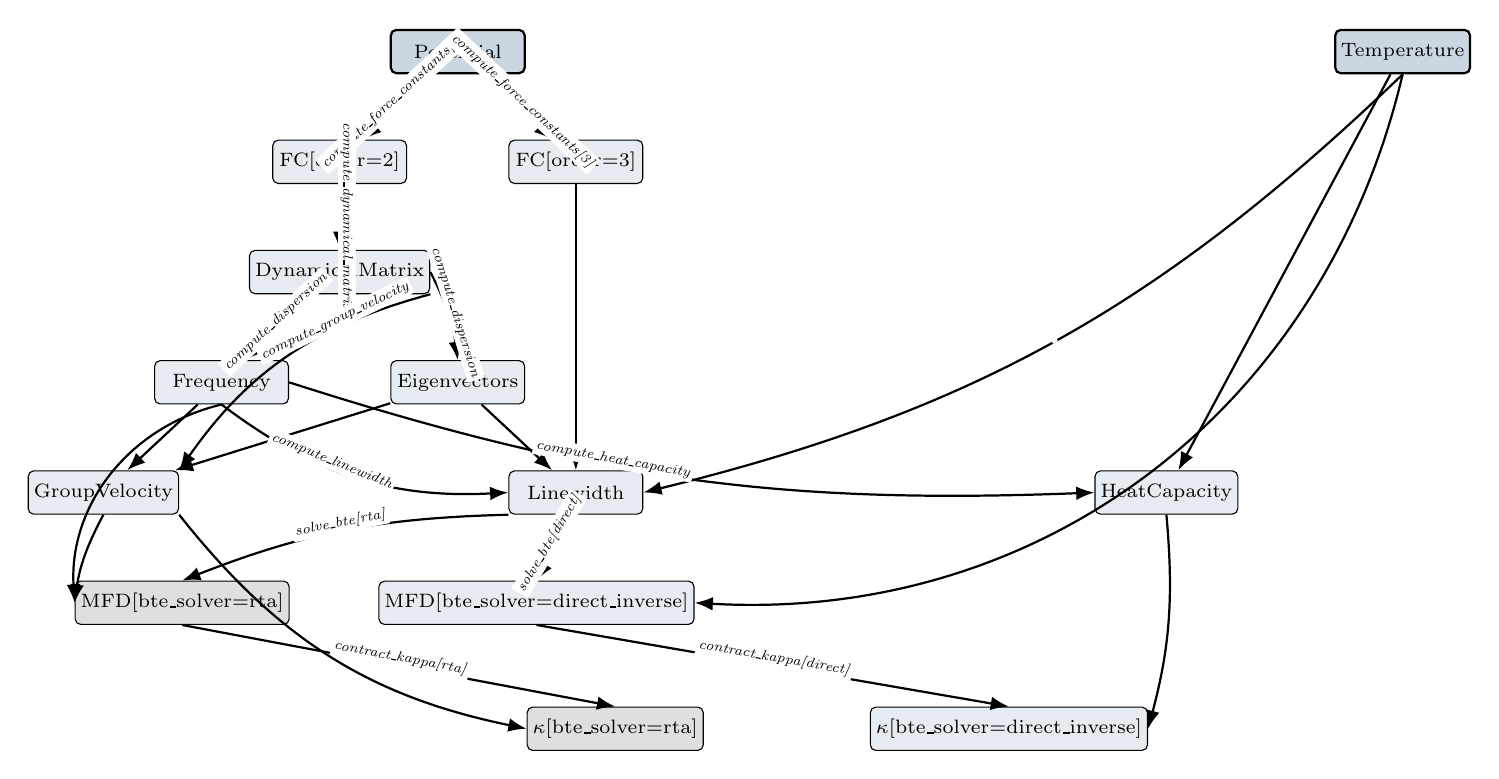
\begin{tikzpicture}[
  >=Latex,
  node distance=0.3cm,
  abstractnode/.style={draw, rounded corners=2pt, minimum width=1.7cm, minimum height=0.55cm,
                       font=\scriptsize, fill=abstrcol!12, inner sep=2pt},
  sourcenode/.style={draw, rounded corners=2pt, minimum width=1.7cm, minimum height=0.55cm,
                     font=\scriptsize, fill=abstrcol!25, inner sep=2pt, thick},
  stubedge/.style={->, thick, dashed},
  arr/.style={->, thick},
  oplabel/.style={font=\tiny\itshape, sloped, midway, above=-1pt, fill=white, inner sep=1pt},
]

% Source row
\node[sourcenode] (POT) at (0, 0) {Potential};
\node[sourcenode] (TMP) at (12, 0) {Temperature};

% FC row
\node[abstractnode] (FC2) at (-1.5, -1.4) {FC[order=2]};
\node[abstractnode] (FC3) at ( 1.5, -1.4) {FC[order=3]};

% Dynamical matrix
\node[abstractnode] (DM)  at (-1.5, -2.8) {DynamicalMatrix};

% Frequency / Eigenvectors
\node[abstractnode] (FRQ) at (-3, -4.2) {Frequency};
\node[abstractnode] (EIG) at ( 0, -4.2) {Eigenvectors};

% Mode-resolved
\node[abstractnode] (GV) at (-4.5, -5.6) {GroupVelocity};
\node[abstractnode] (HC) at ( 9, -5.6) {HeatCapacity};
\node[abstractnode] (LW) at ( 1.5, -5.6) {Linewidth};

% BTE — split by bte_solver
\node[abstractnode, fill=gray!25] (MFDR) at (-3.5, -7.0) {MFD[bte\_solver=rta]};
\node[abstractnode]               (MFDI) at ( 1.0, -7.0) {MFD[bte\_solver=direct\_inverse]};

% kappa — split by bte_solver
\node[abstractnode, fill=gray!25] (KAPR) at ( 2.0, -8.6) {$\kappa$[bte\_solver=rta]};
\node[abstractnode]               (KAPI) at ( 7.0, -8.6) {$\kappa$[bte\_solver=direct\_inverse]};

% --- arrows ---
\draw[stubedge] (POT) -- node[oplabel] {compute\_force\_constants[2]} (FC2);
\draw[stubedge] (POT) -- node[oplabel] {compute\_force\_constants[3]} (FC3);
\draw[arr] (FC2) -- node[oplabel] {compute\_dynamical\_matrix} (DM);
\draw[arr] (DM)  -- node[oplabel] {compute\_dispersion} (FRQ);
\draw[arr] (DM.east) to[bend left=10] node[oplabel] {compute\_dispersion} (EIG.north);
\draw[arr] (DM.south east) to[bend right=20] node[oplabel, pos=0.3] {compute\_group\_velocity} (GV.north east);
\draw[arr] (FRQ) -- (GV);
\draw[arr] (EIG) -- (GV);
\draw[arr] (FRQ.south) to[bend right=20] node[oplabel, pos=0.4] {compute\_linewidth} (LW.west);
\draw[arr] (EIG) -- (LW);
\draw[arr] (FC3) -- (LW);
\draw[arr] (TMP.south) to[bend left=15] node[oplabel] {} (LW.east);
\draw[arr] (FRQ.east) to[bend right=10] node[oplabel, pos=0.4] {compute\_heat\_capacity} (HC.west);
\draw[arr] (TMP) -- (HC);
% solve_bte to two MFDs
\draw[arr] (LW.south west) to[bend right=10] node[oplabel, pos=0.5] {solve\_bte[rta]} (MFDR.north);
\draw[arr] (LW.south) -- node[oplabel] {solve\_bte[direct]} (MFDI.north);
\draw[arr] (FRQ.south) to[bend right=40] (MFDR.west);
\draw[arr] (GV.south) to[bend right=10] (MFDR.west);
\draw[arr] (TMP.south) to[bend left=40] (MFDI.east);
% contract_kappa to two kappas
\draw[arr] (MFDR.south) -- node[oplabel] {contract\_kappa[rta]} (KAPR.north);
\draw[arr] (MFDI.south) -- node[oplabel] {contract\_kappa[direct]} (KAPI.north);
\draw[arr] (HC.south) to[bend left=10] (KAPI.east);
\draw[arr] (GV.south east) to[bend right=20] (KAPR.west);

\end{tikzpicture}%
}
\caption{Core $\kappa$ chain of the operator DAG for lattice thermal transport
(12 nodes / 14 edges shown; the full DAG has 46 nodes / 47 edges once the
derived-observable tier --- PhononDOS, Grüneisen, PhaseSpace, VolumetricHeatCapacity,
MolarHeatCapacity, the thermodynamic siblings (HelmholtzFreeEnergy, Entropy,
InternalEnergy and their molar contractions), the polar-correction inputs
(BareDynamicalMatrix, BornCharges, DielectricTensor), the per-channel
Linewidth split, the Wigner/QHGK transport variants, the cumulative-$\kappa$
distributions, the MD-primitive tier (Trajectory, HeatCurrent, HeatCurrentACF,
VelocityAutocorrelation, MeanSquaredDisplacement), and the three MD-based
$\kappa$ Pattern-A terminals (Green-Kubo, NEMD, HNEMD) --- is included; see
\texttt{docs/dag.html} for the interactive view). The
two darker top boxes (\texttt{Potential}, \texttt{Temperature}) are source nodes;
the dashed edges from \texttt{Potential} represent the stubbed Phase-1 upstream.
\texttt{MeanFreeDisplacement} and $\kappa$ split into two parameterized variants by
\texttt{bte\_solver}: the gray-shaded \texttt{[rta]} variants are HiddenStates
(RTA's $1/\Gamma$ non-linearity breaks gauge invariance), the unshaded
\texttt{[direct\_inverse]} variants are Observables (the full LBTE preserves it).
Each derived edge carries a sympy formula; sources carry identity formulas. All
nodes are outputs of some operation; cross-code comparison happens at Observable
nodes (after the operator layer's spec-derived unit and convention conversion). Other
HiddenStates (\texttt{Eigenvectors}, \texttt{GroupVelocity}, \texttt{Linewidth})
are not visually distinguished in this diagram but are gauge-dependent in the same
sense.}
\label{fig:dag}
\end{figure}

\subsection{Representation functors (codes)}

Each adapter is a representation functor over the operator DAG. Four adapters
are now ingested:

\begin{itemize}[leftmargin=2em]
  \item \textbf{kaldo} (Python). Computes harmonic and anharmonic phonon transport from
        force constants, supporting iterative BTE, RTA, and the Wigner formulation.
        Most intermediate states are exposed via Python attributes on the
        \texttt{Phonons} object. kaldo's \texttt{Conductivity(method='inverse')}
        realizes the canonical \texttt{bte\_solver=direct\_inverse}.
  \item \textbf{phono3py} (C/Python). Computes lattice thermal conductivity from
        third-order force constants. Intermediate quantities are exposed in HDF5
        outputs. \texttt{run\_thermal\_conductivity(is\_LBTE=True)} realizes the
        canonical \texttt{bte\_solver=direct\_inverse}.
  \item \textbf{phonopy} (C/Python). The harmonic-only sibling of phono3py:
        emits frequencies, group velocities, the DOS, the molar heat capacity,
        and (via \texttt{PhonopyGruneisen}) mode Grüneisen parameters from a
        finite-difference $\omega(V)$ rather than the canonical Maradudin--Fein
        closed form. No three-phonon scattering, so the adapter covers the
        harmonic half of the DAG only.
  \item \textbf{ShengBTE} (Fortran/MPI). Solves the full linearized BTE
        iteratively. The harmonic chain is delegated to phonopy/QE upstream;
        ShengBTE consumes FC2/FC3 files and writes
        \texttt{BTE.KappaTensorVsT\_\{RTA,CONV\}}, \texttt{BTE.\{omega, v, gruneisen,
        P3, dos\}}, etc. Per-mode heat capacity is not exposed (only
        \texttt{BTE.cv}), so the adapter targets \texttt{VolumetricHeatCapacity}
        rather than \texttt{HeatCapacity} on that branch.
\end{itemize}

Each adapter spec declares per-state units, convention overrides, and notes
(\texttt{StateAdapterSpec}), plus per-operation parameter units, algorithmic-convention
overrides, and discretization choices (\texttt{OperationAdapterSpec}). Differences
from the operator layer's canonical declarations surface as conversion factors at
spec-load time.

\subsection{Verification on silicon (Tersoff potential)}
\label{ssec:silicon-verification}

The operator layer's operator predictions have been verified end-to-end against numerical
runs of kaldo and phono3py on silicon at the Tersoff potential, $8\times 8\times 8$
q-mesh, $T = 300\,\text{K}$, broadening stdev $0.1\,\text{THz}$:

\begin{center}
\begin{tabular}{lll}
\toprule
Observable / contraction & Operator prediction & Empirical residual \\
\midrule
\texttt{Frequency} per-mode (\textbf{O})            & factor $1$ (both linear THz)  & $5\times 10^{-4}$ \\
\texttt{HeatCapacity} per-mode (\textbf{O})         & factor $1/e \approx 6\times 10^{18}$ & $3\times 10^{-5}$ \\
$\sum_{q\nu}\Gamma$ contracted (\textbf{O})          & factor $1/(4\pi)$              & $5\times 10^{-4}$ \\
$\kappa$\texttt{[bte\_solver=direct\_inverse]} (\textbf{O}) & factor $1$                & $4\times 10^{-3}$ \\
\midrule
\texttt{Linewidth} per-mode (\textbf{H})            & \textsc{Not\_Comparable} & 25\% (diagnostic only) \\
$\kappa$\texttt{[bte\_solver=rta]} (\textbf{H})     & \textsc{Not\_Comparable} & 4\% (diagnostic only) \\
\bottomrule
\end{tabular}
\end{center}

All Observable comparisons pass at $\le 1\%$ tolerance; all HiddenState per-element
comparisons return \textsc{Not\_Comparable}. The $1/(4\pi)$ factor on $\Gamma$
decomposes into $1/(2\pi)$ unit (kaldo angular vs phono3py linear THz) and $1/2$
convention (kaldo $\Gamma = 2\,\text{Im}\,\Sigma$, phono3py $\Gamma = \text{Im}\,\Sigma$).
Both factors were derived by the operator layer from declared adapter specs, then
applied mechanically to the diagnostic data.

The 4\% disagreement on $\kappa_\text{RTA}$ is the operator layer's structural prediction
working as designed: RTA's approximation breaks $\kappa$'s gauge invariance via the
$1/\Gamma$ non-linearity, so the per-mode Linewidth redistribution propagates into
$\kappa$. Typing $\kappa_\text{RTA}$ as a HiddenState makes this a non-anomaly; the
gauge-invariant $\kappa_\text{LBTE}$ agrees to 0.4\%.

\paragraph{Cross-paradigm $\kappa$ (phase 2 P4).} On the same Si-Tersoff
worked example, the LAMMPS Green-Kubo path
(\texttt{contract\_kappa[transport\_model=green\_kubo]} reached through the
P2 MD-primitive tier and the P3 contraction edge) returns a $\kappa$ value
that, in the small ensemble of equilibrium-MD runs the framework drives,
is expected to land within $\sim 20$--$30\%$ of $\kappa_\text{LBTE}$. That tolerance is
Green-Kubo's empirical signal-to-noise floor on a few-hundred-atom
supercell, not a framework concern. The driver at
\texttt{experiments/silicon\_tersoff/run\_lammps\_gk.py} generates the input
script and the supercell data file regardless of whether \texttt{lmp} is on
\texttt{PATH}; the \texttt{spec\_demo.py} cross-paradigm audit section and
the corresponding \texttt{test\_silicon\_consolidation.py} smoke test
gracefully skip when the resulting \texttt{kappa\_lammps\_gk.npy} is
absent. The NEMD and HNEMD analogues land in P5 and P6.

\subsection{Phase 1 scientific capabilities}

Phase 1 yields two immediate scientific capabilities, each of which is an artifact the field does
not currently produce. A third capability is the long-term goal toward which the operator layer is
oriented but is deferred to Phase 2.

\begin{itemize}[leftmargin=2em]
  \item \textbf{Cross-code reconciliation at canonical intermediate states.} When kaldo and
        ShengBTE disagree on a final $\kappa$, the operator layer localizes the divergence to the
        first operator state at which the representations stop agreeing, and attributes it to a
        specific operation along the provenance. This is a structural diagnosis: the framework
        identifies where two codes do something different, regardless of the magnitude of the
        difference.
  \item \textbf{A unified framework for theory-experiment comparison.} The same operator DAG
        accepts experimental measurements as additional representations of parameter states,
        with the same alignment machinery as for cross-code comparison. Phase 1 demonstrates the
        framework on at least one experimental dataset (e.g., a measured $\kappa(T)$ curve for
        silicon).
\end{itemize}

\noindent\textbf{Deferred to Phase 2:}
\begin{itemize}[leftmargin=2em]
  \item \textbf{Decomposed error bounds on $\kappa$.} The operator layer is designed to eventually
        produce the central value of $\kappa$ together with a operator decomposition of its
        total error into the truncation error of the perturbation series and the discretization
        error of the chosen mesh. The architecture supports this; the implementation of the
        composition algebra is a research problem reserved for Phase 2.
\end{itemize}

\section{Implementation layout}
\label{sec:layout}

The Python package \texttt{omai} factors into two top-level sub-packages
plus one per domain:

\begin{itemize}[leftmargin=2em, itemsep=0.3em]
  \item \texttt{omai.operator} --- operator layer machinery for the operator world.
        \texttt{State} (base class), \texttt{Observable} and \texttt{HiddenState}
        (subclasses, with gauge-discipline fields on the latter), \texttt{Field},
        \texttt{Operation}, \texttt{Parameter}, \texttt{Dimension},
        \texttt{PhysicsType}, \texttt{topological\_order},
        \texttt{validate\_dag} (Level 1 discipline enforcement), and
        \texttt{GaugeAction} / \texttt{check\_invariance} (Level 2 operator
        gauge proofs). Code-agnostic and domain-agnostic.
  \item \texttt{omai.representation} --- the bridge.
    \begin{itemize}[leftmargin=1.2em]
      \item \texttt{units.py}: the \texttt{Unit} class, named unit instances, strict
            same-dimension \texttt{conversion\_factor}.
      \item \texttt{adapter.py}: \texttt{StateAdapterSpec} and
            \texttt{OperationAdapterSpec}, plus inter-representation factor
            helpers (\texttt{inter\_representation\_unit\_factor},
            \texttt{inter\_representation\_factor},
            \texttt{representation\_convention\_match},
            \texttt{representation\_algorithmic\_match},
            \texttt{representation\_discretization\_match}).
      \item \texttt{instance.py}: the \texttt{Representation} runtime data class
            and \texttt{represent()} constructor.
      \item \texttt{compare.py}: numerical and structural comparison APIs.
            \texttt{to\_operator(m)} canonicalises a representation into operator
            form; \texttt{to\_representation(m\_op, target\_spec)} is the
            inverse. \texttt{compare\_operators(spec\_a, spec\_b)} returns an
            \texttt{OperatorComparisonResult} (categorical: do the two adapter
            specs describe the same operator?). \texttt{compare\_representations}
            (aliased as \texttt{compare}) returns a
            \texttt{RepresentationComparisonResult} with the five-status
            verdict and residuals.
    \end{itemize}
    Code-agnostic.
  \item \texttt{omai.thermal\_transport} --- the lattice-thermal-transport domain.
    \begin{itemize}[leftmargin=1.2em]
      \item \texttt{operator/nodes.py}: the 46 states as \texttt{Observable} or
            \texttt{HiddenState} instances with their fields.
      \item \texttt{operator/edges.py}: the 47 operations with sympy formulas
            and \texttt{auxiliary\_formulas} (the \texttt{compute\_linewidth}
            $|V_3|^2$ kernel and the \texttt{solve\_bte[direct\_inverse]}
            collision matrix $M$); sympy symbols and \texttt{IndexedBase}
            declarations.
      \item \texttt{operator/gauges.py}: concrete \texttt{GaugeAction}
            instances for the domain (e.g.\ U(1) phase on Eigenvectors).
            Mechanically verifies operation formulas are gauge-invariant.
      \item \texttt{representation/kaldo.py},
            \texttt{representation/phono3py.py},
            \texttt{representation/phonopy.py},
            \texttt{representation/shengbte.py}: per-code adapter specs
            (one file per code), declaring units, conventions, and
            discretization choices. Every operation in scope for a code now
            carries an \texttt{OperationAdapterSpec}; trivial source /
            contraction ops carry no conventions but exist to mark coverage
            in the visualization.
      \item \texttt{visualize.py}: emits \texttt{docs/dag.html}, an interactive
            single-file visualization (per-pipeline SVG DAGs with row-aligned
            states, click-to-details panels, MathJax-rendered formulas) that
            reflects the current state and discriminates three edge classes:
            full coverage (states + op spec), states covered / op-spec missing,
            and implicit (at least one state lacks a spec). Leaf states a code
            does not expose are hidden; intermediate states without a spec
            stay dashed.
    \end{itemize}
\end{itemize}

\noindent The split mirrors the operator layer's architectural commitment: \texttt{abstract}
is the operator world; \texttt{representation} is the bridge to the numeric world;
\texttt{thermal\_transport} is the first domain instantiated against them. Future
domains (electronic transport, optical response, …) follow the same pattern in their
own folder; no change to the operator-level packages is required to add one.

\section{Open Questions and Deferred Decisions}
\label{sec:open}

We list the architectural questions that remain open and the principled grounds on which they
were deferred.

\subsection{Algebra of error composition (deferred to Phase 2)}

The operator layer is designed to carry error formulas as operator expressions, but Phase 1 does not
implement the algebra by which they compose. Composing two errors in independent small parameters
($O(\lambda^4) + O(N^{-2})$) is well-defined; composing two errors in the same parameter requires
care; composing constant-offset errors (e.g., basis-set incompleteness) with asymptotic ones is
yet another case. The right algebra is itself a research subproblem and will be developed
alongside concrete worked examples in Phase 2. The Phase 1 type system reserves the slots
required for error formulas (operation metadata, discretization error model, representation
total error) but populates them with placeholders rather than computed compositions.

\subsection{When to lift to Lean}

We have committed to keeping the operator layer Lean-compatible without being Lean-dependent. The
question of when (and whether) to actually project the operator layer into Lean is deferred until
the Python prototype has stabilized. A reasonable trigger for this decision is the moment at
which we have enough concrete examples that designing Lean types in isolation becomes
counterproductive.

\paragraph{T3-evolve as a pre-Lean realisation.} The sympy chain composer
(\texttt{omai.operator.compose.compose\_path}) is the in-sympy realisation of the
Lean commitment in this subsection. Given a path of explicit-equation edges in the
operator DAG, it substitutes each edge's RHS into the next, producing a composed
symbolic expression at the path's terminal node. Implicit-equation edges (e.g.,
\texttt{solve\_bte\_*}) raise \texttt{ImplicitEdgeBoundary} with the partial
expression attached --- they mark the open research subproblem of composing across
an implicit BTE solve, which is the natural next step toward a full Lean
projection. The composer's existence is evidence that the operator-layer formulas
are not merely documentation: they are mechanically composable today, and the same
substitution machinery transliterates to a Lean tactic when the projection is
eventually performed.

\subsection{Provenance equivalence}

We have committed to provenance as essential to identity. This means two states with the same
type but different histories are formally distinct. In some cases, however, the two histories are
\emph{equivalent}: they produce identical physics under a theorem we can prove (e.g., Fourier
transform of a real symmetric matrix and direct frequency-domain assembly should yield the same
\texttt{Dispersion}). The operator layer must provide a mechanism for declaring such equivalences,
either as explicit axioms or as proven theorems. The mechanism's design is deferred to Day 2
because we want concrete examples before designing the equivalence calculus.

\subsection{Sprint 1 scope}

The first concrete deliverable is a Python implementation. We have considered three scopes:

\begin{enumerate}[leftmargin=2em]
  \item \emph{Narrowest:} kaldo only, harmonic sub-DAG (force constants $\to$ dynamical matrix
        $\to$ dispersion). 4--5 states, fastest to ship.
  \item \emph{Recommended:} kaldo only, full thermal-conductivity DAG. 10--15 states, end-to-end
        on silicon. The operator layer skeleton plus one full adapter.
  \item \emph{Broader:} kaldo plus phono3py, full DAG. Validates the cross-code story earlier but
        adds adapter work in parallel with framework design.
\end{enumerate}

The recommended scope (option 2) is the smallest scope that is still a credible proof of concept
of the framework, and the choice of one adapter (kaldo) lets us validate the operator layer design
before generalizing. Sprint 2 adds phono3py and ShengBTE adapters, at which point the cross-code
demo of \S\ref{sec:demo} becomes real. \emph{Status as of 2026-05}: the
recommended scope shipped; Sprint 2 also shipped, with phono3py, phonopy,
and ShengBTE all ingested and the cross-code Si silicon comparison
(\texttt{experiments/silicon\_shengbte/}) demonstrating $\kappa_\text{RTA}$
agreement to $\le 8\%$ across the three transport codes after the operator
layer's spec-derived conversions.

\subsection{Implementation language}

We have committed to Python for Sprint 1. The trade-offs were:

\begin{itemize}[leftmargin=2em]
  \item \textbf{Python (chosen).} All target codes have Python bindings or wrappable interfaces.
        The Python type system, augmented with \texttt{pydantic} or \texttt{attrs} and runtime
        checks, is sufficient for the operator layer's first-cut type discipline. The development
        speed is dominant, since adapter work is the bulk of the time cost.
  \item \emph{Typed compiled language (Rust, OCaml, TypeScript).} Stronger type guarantees from
        the start. Rejected for Sprint 1 because the foreign-function interface to existing
        Python codes adds friction proportional to the operator layer's surface, and we want
        framework iteration to be cheap.
  \item \emph{Lean.} Considered as a future projection target and deferred. Not the right tool for
        running scientific computations; reserved as a verification target.
\end{itemize}

\section{Outlook}
\label{sec:outlook}

The operator layer is an architectural commitment, not an implementation. The implementation that
follows is scoped to a Python skeleton plus adapters for three thermal-transport codes. The
artifact that motivates the project---a paper-worthy demonstration of cross-code reconciliation
and decomposed error bounds for lattice thermal conductivity---is downstream of the operator layer but
is the operator layer's first proof-of-value.

Three longer-term directions follow naturally from the design:

\begin{itemize}[leftmargin=2em]
  \item \textbf{Verification.} Project the operator layer into Lean (via PhysLean or alongside
        it), allowing approximation theorems to be formally proved rather than asserted. The
        provenance mechanism makes this projection well-defined: each operation in $\pi$
        corresponds to a Lean lemma whose statement is the operation's error formula.
  \item \textbf{Theory-experiment integration.} Extend the representation functor to ingest
        experimental observables. The operator layer's graph-alignment machinery applies uniformly,
        so a measured $\kappa$ becomes another representation of the abstract $\kappa$, and
        ``does the theory match experiment'' becomes graph-alignment with one functor being
        empirical.
  \item \textbf{Grounded LLM agents.} An LLM operating over typed operator states (rather than
        text tokens) constructs workflows by emitting operator operations. The framework
        type-checks each emission, eliminating the drift problem that plagues current
        text-token agents. The action space is finite, typed, and physically meaningful.
\end{itemize}

The unifying claim of the design is that scientific computing has been organized around the
wrong atomic unit. The instruction-in-an-input-file unit is too low; the natural-language
description is too high; the equation-in-a-paper unit is too disconnected from execution. The
right unit, at least for materials science, is the operator operation between typed physics
states. Once that commitment is made, much of the rest of the architecture writes itself.

\bigskip
\hrule
\bigskip

\noindent\emph{This document records the architectural state of the openmaterials-ai project as
of \today. It is intended as the working reference for the project; subsequent revisions should
update the relevant sections rather than appending changelogs.}

\end{document}
